%%%%%%%%%%%%%%%%%%%%%%%%%%%%%%%%%%%%%%%%%%%%%%%%%%%%%%%%%%%%%%%%%%%%%%%%%%%%%%%%%%
\begin{frame}[fragile]\frametitle{}
\begin{center}
{\Large Cypher}
\end{center}
\end{frame}


%%%%%%%%%%%%%%%%%%%%%%%%%%%%%%%%%%%%%%%%%%%%%%%%%%%%%%%%%%%
\begin{frame}[fragile]\frametitle{Introduction}
A pattern matching query language made for graphs

\begin{itemize}
\item Declarative: say, what you want? and not how to search for the answer (Imperative)
\item Expressive
\item Pattern-Matching : ASCI Art
\end{itemize}

\end{frame}


%%%%%%%%%%%%%%%%%%%%%%%%%%%%%%%%%%%%%%%%%%%%%%%%%%%%%%%%%%%
\begin{frame}[fragile]\frametitle{Basic Syntax}

\begin{center}
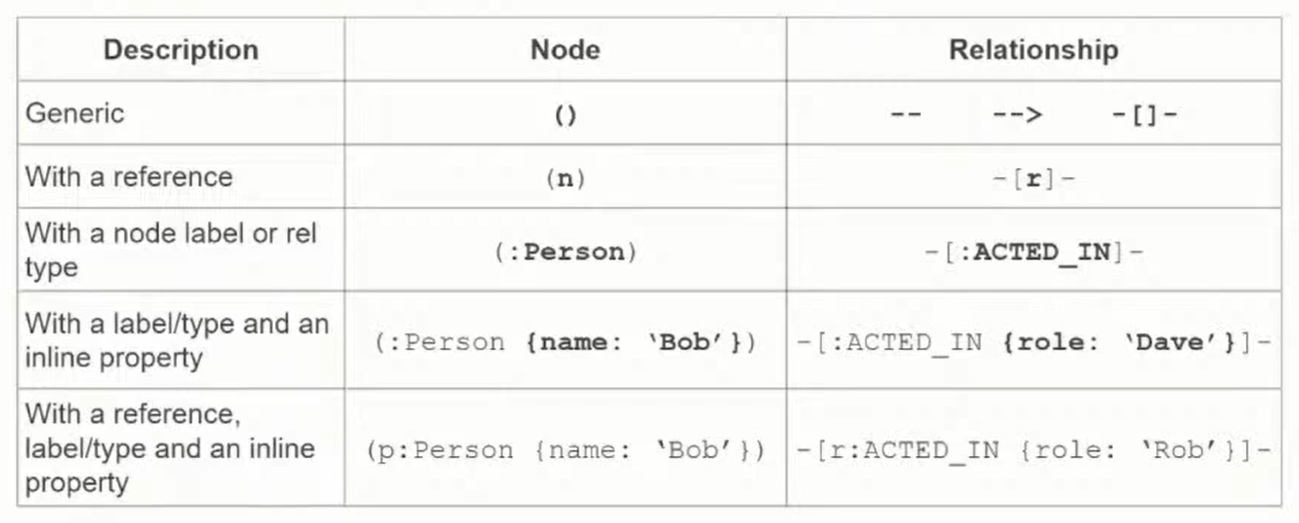
\includegraphics[width=\linewidth,keepaspectratio]{neo4j9}
\end{center}	  


{\tiny (Ref: Introduction to Neo4j - a hands-on crash course  - neo4j)}

\end{frame}


%%%%%%%%%%%%%%%%%%%%%%%%%%%%%%%%%%%%%%%%%%%%%%%%%%%%%%%%%%%
\begin{frame}[fragile]\frametitle{MATCH}

Retrieve nodes

\begin{center}
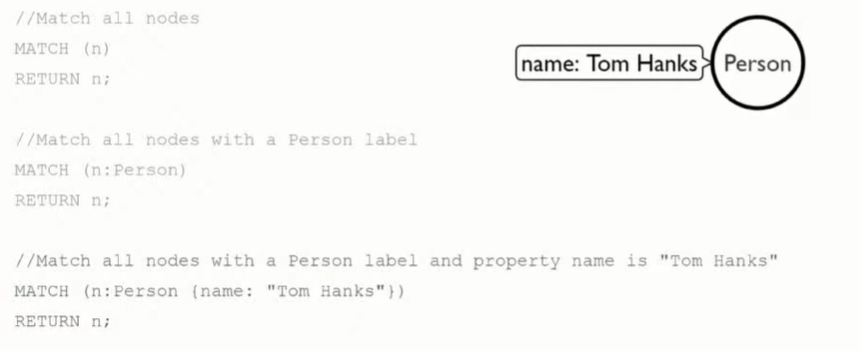
\includegraphics[width=\linewidth,keepaspectratio]{neo4j10}
\end{center}	  


{\tiny (Ref: Introduction to Neo4j - a hands-on crash course  - neo4j)}

\end{frame}

%%%%%%%%%%%%%%%%%%%%%%%%%%%%%%%%%%%%%%%%%%%%%%%%%%%%%%%%%%%
\begin{frame}[fragile]\frametitle{MATCH}

Retrieve nodes with properties

\begin{center}
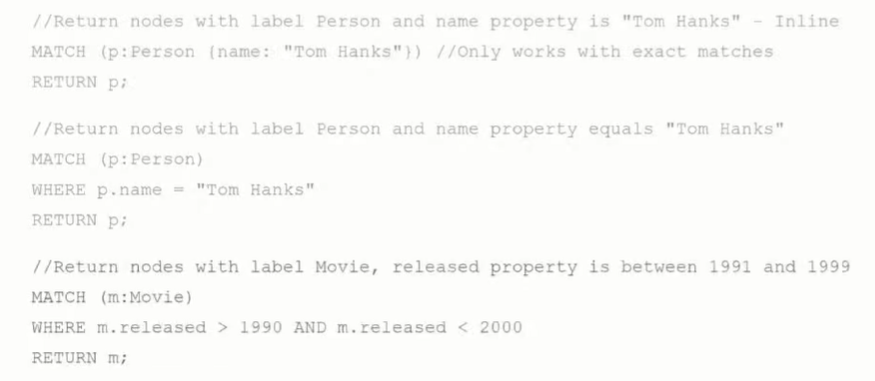
\includegraphics[width=\linewidth,keepaspectratio]{neo4j11}
\end{center}	  


{\tiny (Ref: Introduction to Neo4j - a hands-on crash course  - neo4j)}

\end{frame}

%%%%%%%%%%%%%%%%%%%%%%%%%%%%%%%%%%%%%%%%%%%%%%%%%%%%%%%%%%%
\begin{frame}[fragile]\frametitle{MATCH}

Retrieve nodes with relationships

\begin{center}
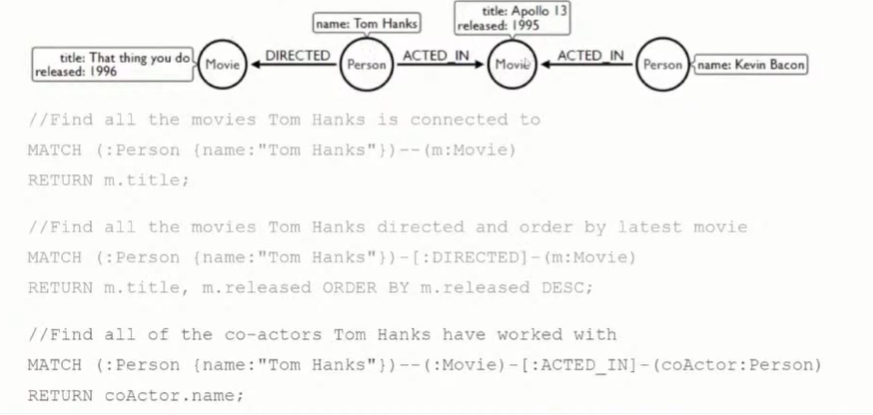
\includegraphics[width=\linewidth,keepaspectratio]{neo4j12}
\end{center}	  


{\tiny (Ref: Introduction to Neo4j - a hands-on crash course  - neo4j)}

\end{frame}

%%%%%%%%%%%%%%%%%%%%%%%%%%%%%%%%%%%%%%%%%%%%%%%%%%%%%%%%%%%
\begin{frame}[fragile]\frametitle{CREATE}

 Creating new nodes
 

\begin{center}
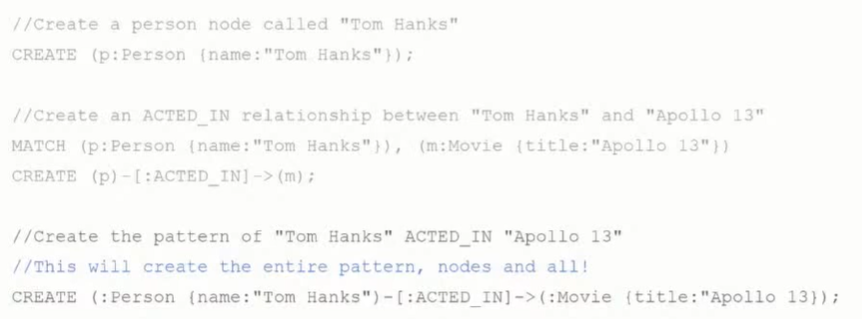
\includegraphics[width=\linewidth,keepaspectratio]{neo4j13}
\end{center}	  


{\tiny (Ref: Introduction to Neo4j - a hands-on crash course  - neo4j)}

\end{frame}

%%%%%%%%%%%%%%%%%%%%%%%%%%%%%%%%%%%%%%%%%%%%%%%%%%%%%%%%%%%
\begin{frame}[fragile]\frametitle{Example}
A Social Recommendation

\begin{center}
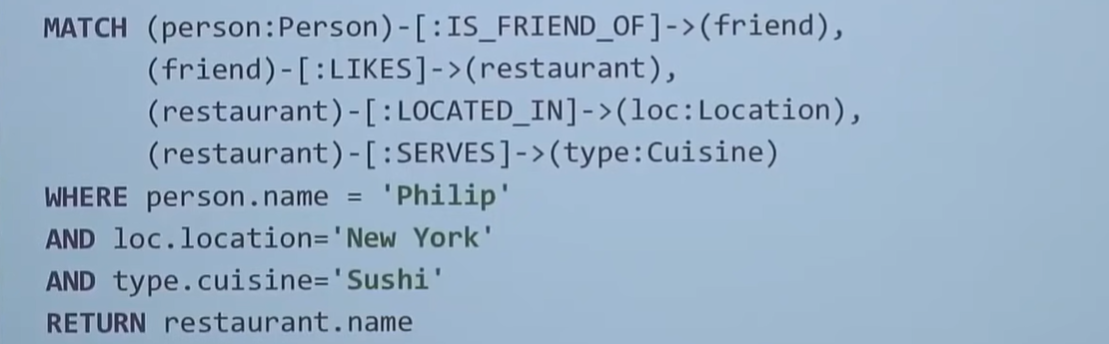
\includegraphics[width=\linewidth,keepaspectratio]{neo4j15}
\end{center}	  


{\tiny (Ref: Introduction to Neo4j and Graph Databases
 - M David Allen)}

\end{frame}

%%%%%%%%%%%%%%%%%%%%%%%%%%%%%%%%%%%%%%%%%%%%%%%%%%%%%%%%%%%
\begin{frame}[fragile]\frametitle{Aggregates}
No need to specify grouping key

\begin{lstlisting}
// implicitly groups by p.name
MATCH (p.Person)-[:ACTED_IN]->(m:Movie)
RETURN p.name, count(*) AS numberOfMovies
\end{lstlisting}	  

There is no group-by statement. Other Aggregates are SUM, STDDEV, etc.

{\tiny (Ref: Introduction to Neo4j and Graph Databases
 - M David Allen)}

\end{frame}

%%%%%%%%%%%%%%%%%%%%%%%%%%%%%%%%%%%%%%%%%%%%%%%%%%%%%%%%%%%
\begin{frame}[fragile]\frametitle{Constrains}
Unique

\begin{lstlisting}
// to ensure uniqueness and fast lookups
CREATE CONSTRAINT ON (label:Label)
ASSERT label.property IS QUNIQUE
\end{lstlisting}	  

{\tiny (Ref: Introduction to Neo4j and Graph Databases
 - M David Allen)}

\end{frame}

%%%%%%%%%%%%%%%%%%%%%%%%%%%%%%%%%%%%%%%%%%%%%%%%%%%%%%%%%%%
\begin{frame}[fragile]\frametitle{Indexes}
Used only to find the starting points for queries

\begin{center}
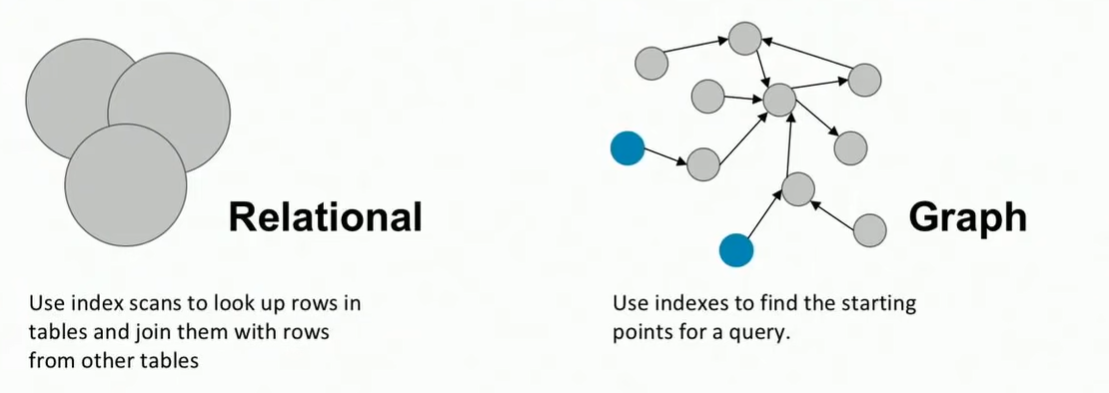
\includegraphics[width=\linewidth,keepaspectratio]{neo4j16}
\end{center}	  


{\tiny (Ref: Introduction to Neo4j and Graph Databases
 - M David Allen)}

\end{frame}

%%%%%%%%%%%%%%%%%%%%%%%%%%%%%%%%%%%%%%%%%%%%%%%%%%%%%%%%%%%
\begin{frame}[fragile]\frametitle{Example}
What are the top 10 jobs for me, that are same location as I am in and also for which I have necessary qualifications?

\begin{center}
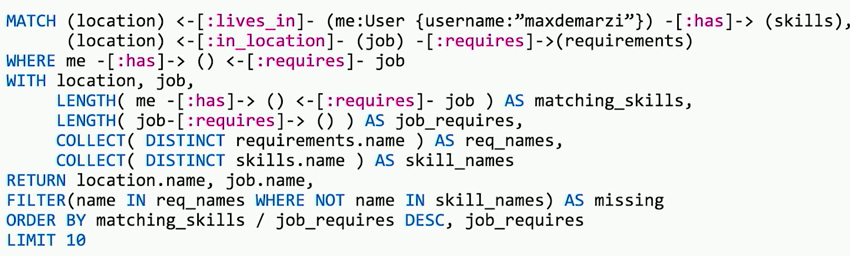
\includegraphics[width=\linewidth,keepaspectratio]{neo4j27}
\end{center}	    



{\tiny (Ref: Secret Sauce of Neo4j: Modeling and Querying Graphs
 - Max De Marzi )}

\end{frame}

%%%%%%%%%%%%%%%%%%%%%%%%%%%%%%%%%%%%%%%%%%%%%%%%%%%%%%%%%%%
\begin{frame}[fragile]\frametitle{Answer}

Partial sub-graph match

\begin{center}
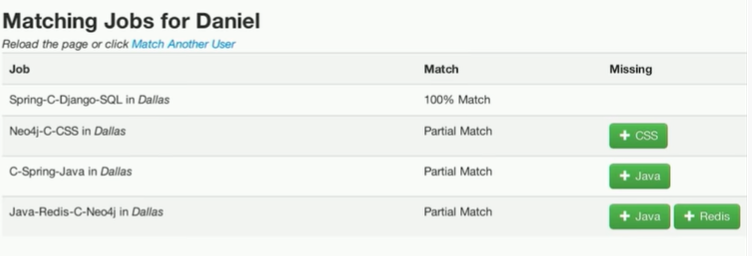
\includegraphics[width=\linewidth,keepaspectratio]{neo4j28}
\end{center}	    


{\tiny (Ref: Secret Sauce of Neo4j: Modeling and Querying Graphs
 - Max De Marzi )}

\end{frame}

%%%%%%%%%%%%%%%%%%%%%%%%%%%%%%%%%%%%%%%%%%%%%%%%%%%%%%%%%%%%%%%%%%%%%%%%%%%%%%%%%%
\begin{frame}\frametitle{Tips, Think in Patterns}


\begin{itemize}
\item  Drop the WHERE clause
\item  Adopt the MATCH clause
\end{itemize}


{\tiny (Ref: CIS 6930 - Advanced Databases - Neo4j )}
\end{frame}





